\documentclass[hidelinks]{ctexart}

\usepackage{van-de-la-illinoise}

\title{引力波的产生及其探测}
\date{}
\author{18级少年班学院\quad PB18000112\quad 陈泽}

\DeclareSIUnit{\parsec}{pc}
\DeclareSIUnit{\year}{yr}
\DeclareSIUnit{\lightyear}{l.y.}
\def\sun{\odot}
\hypersetup{citecolor=black}

\begin{document}

\maketitle

\section{引力波的产生} % (fold)
\label{sec:引力波的产生}

\subsection{弱场下的Einstein方程} % (fold)
\label{sub:弱场下的einstein方程}

完整的Einstein场方程为(全文使用自然单位制)
\[ G^{\mu\nu} = R^{\mu\nu} - \half R g_{\mu\nu} = 8\pi T^{\mu\nu}. \]
在弱场近似下设
\[ g_{\mu\nu} = \eta_{\mu\nu} + h_{\mu\nu}, \]
其中$\eta$是通常的Minkowski度规, 号差$\pare{-,+,+,+}$, 而$\abs{h_{\mu\nu}}\ll 1$是微扰. 由此可得Riemann张量
\[ R_{\alpha\beta\mu\nu} = \half\pare{h_{\alpha\nu,\beta\mu} + h_{\beta\mu,\alpha\nu} - h_{\alpha\mu,\beta\nu} - h_{\beta\nu,\alpha\mu}}. \]
其中逗号表示对某一坐标的偏微分. 通过坐标变换
\[ x'^\alpha = x^\alpha + \xi^\alpha\pare{x^\beta}, \]
可得相应的$h$的分量的变换为(一阶近似下)
\[ h_{\mu\nu} \rightarrow h_{\mu\nu} - \xi_{\mu,\nu} - \xi_{\nu,\mu}. \]
这一变换称为规范变换, \textbf{Riemann张量在这一规范变换下不变}. 定义
\[ \conj{h}^{\mu\nu} = h^{\mu\nu} - \half \eta^{\mu\nu}h,\quad h = {h^\alpha}_\alpha, \]
可以选取适当的$\xi$使得$h$满足Lorentz规范
\[ {\conj{h}^{\mu\nu}}_{,\nu} = 0, \]
则此时
\[ G_{\mu\nu} = -\half\brac{ {\conj{h}_{\mu\nu,\alpha}}^{,\alpha} + \eta_{\mu\nu}{\conj{h}_{\alpha\beta}}^{,\alpha\beta} - {\conj{h}_{\mu\alpha,\nu}}^{,\alpha} - {\conj{h}_{\nu\alpha,\mu}}^{,\alpha} + O\pare{h_{\mu\nu}^2} } = -\half \Box^2 \conj{h}_{\mu\nu}. \]
其中
\[ f^{,\mu} = \eta^{\mu\nu}f_{,\nu} \]
是针对协变坐标的导数而
\[ \Box^2 = \pare{-\+D{t^2}D{^2} + \laplacian} \]
是D'Alembert算子. 此时Einstein场方程近似为
\[ \Box^2 \conj{h}^{\mu\nu} = -16\pi T^{\mu\nu}. \]
在真空下, $T^{\mu\nu} \equiv 0$, 方程变为
\[ \boxed{\Box^2 \conj{h}^{\mu\nu} = 0.} \]
这表明$\conj{h}^{\mu\nu}$每个分量皆满足波动方程.

% subsection 弱场下的einstein方程 (end)

\subsection{平面波解} % (fold)
\label{sub:平面波解}

\subsubsection{TT规范坐标系下的解} % (fold)
\label{ssub:tt规范坐标系下的解}

寻求如下形式
\[ \conj{h}^{\mu\nu} = A^{\mu\nu} \exp\pare{ik_\alpha x^\alpha} \]
的解, 直接代入波动方程可得
\[ k^\alpha k_\alpha = 0, \]
即$k$必定为类光矢量. 因此有诸多和电磁波类似的性质, 例如传播速度为光速. 若记$\omega = k^0$, $\+vk = \pare{k^1,k^2,k^3}$, 则有
\[ \omega^2 = \abs{\+vk}^2. \]
并且注意到Lorentz规范要求
\[ A^{\mu\nu}k_\nu = 0. \]
可以证明通过选取适当的规范变换, 可以同时要求\cite{Schutz2009}
\[ {A^\mu}_\mu = 0,\quad A_{\mu\nu} U^\nu = 0. \]
即\textbf{无迹横波规范}(\textbf{TT规范}), 其中$U^\nu$为任意固定的四维速度. 在这一规范下,
\[ \conj{h}_{\mu\nu}^{\mathrm{TT}} = {h}_{\mu\nu}^{\mathrm{TT}}. \]
选择$U^\nu = \delta^\nu_0$, 并且旋转坐标轴令$k = \pare{\omega,0,0,\omega}$, 则由TT规范可得
\[ \boxed{A_{\mu\nu}^{\mathrm{TT}} = \begin{pmatrix}
    0 & 0 & 0 & 0 \\
    0 & A_{xx} & A_{xy} & 0 \\
    0 & A_{xy} & -A_{xx} & 0 \\
    0 & 0 & 0 & 0
\end{pmatrix}.} \]
在这一坐标系下, 时空仅在$x$-$y$平面内发生弯曲.

% subsubsection tt规范坐标系下的解 (end)

\subsubsection{引力波的偏振} % (fold)
\label{ssub:引力波的偏振}

\begin{figure}[ht]
    \centering
    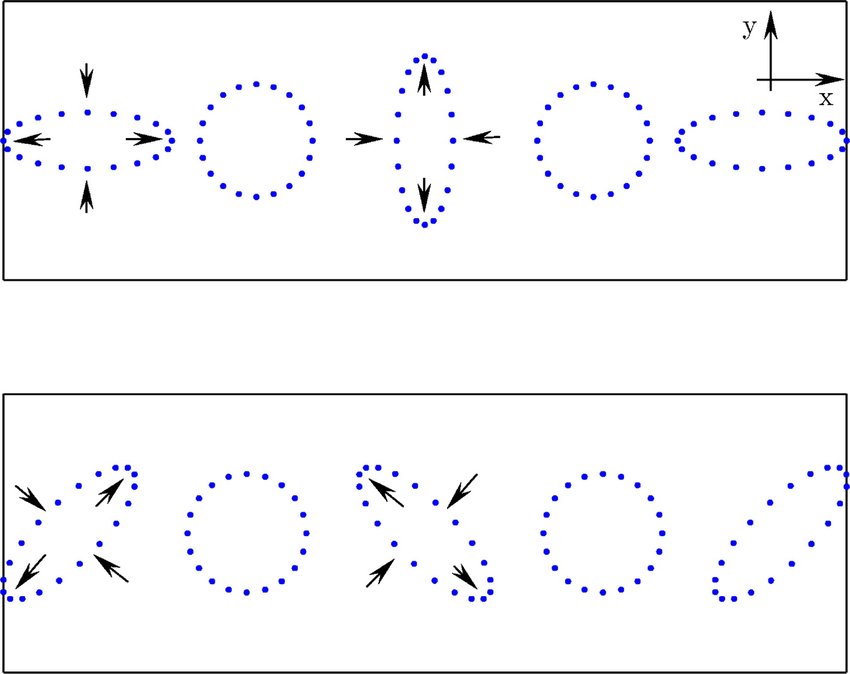
\includegraphics[width=10cm]{src/The-effect-of-a-passing-gravitational-wave-on-a-ring-of-freely-falling-test-particles.png}
    \caption{十字型偏振(上方)和交叉型偏振(下方)的示意图\cite{HGPM}}
    \label{fig:引力波偏振的示意图}
\end{figure}
如果
\[ h^{\mathrm{TT}}_{xx} = -h^{\mathrm{TT}}_{yy} \neq 0,\quad h^{\mathrm{TT}}_{xy} = h^{\mathrm{TT}}_{yx} = 0 \]
则引力波是\textbf{十字型偏振}的. 如果
\[ h^{\mathrm{TT}}_{xy} = h^{\mathrm{TT}}_{yx} \neq 0,\quad h^{\mathrm{TT}}_{xx} = -h^{\mathrm{TT}}_{yy} = 0, \]
则引力波是\textbf{交叉型偏振}的. 示意图如\cref{fig:引力波偏振的示意图}所示, 质点在图中的距离根据其四维固有距离确定. 在TT规范下沿$z$传播的引力波可视为这两种偏振的叠加.

% subsubsection 引力波的偏振 (end)

% subsection 平面波解 (end)

\subsection{平面引力波的物理效应} % (fold)
\label{sub:平面引力波的物理效应}

\subsubsection{TT规范坐标系中的效应} % (fold)
\label{ssub:tt规范坐标系中的效应}

质点沿测地线运动, 满足
\[ \+d\tau d{} U^\alpha + {\Gamma^\alpha}_{\mu\nu}U^\mu U^\nu = 0, \]
若质点于初始时刻静止, 则初始时刻其加速度为(在TT规范确定的坐标系中)
\[ \pare{\+d\tau d{U^\alpha}}_0 = -{\Gamma^\alpha}_{\mu\nu} = -\half e^{\alpha\beta}\pare{h_{\beta 0,0} + h_{0\beta, 0} - h_{00,\beta}} = 0. \]
因此质点(在TT规范确定的坐标系中)将一直维持静止. 尽管如此, 这并不意味着引力波不产生任何效应. 如果考虑两个邻近质点的四维固有距离, 一个位于$\pare{x,y,z} = \pare{0,0,0}$, 一个位于$\pare{x,y,z} = \pare{\epsilon,0,0}$, 则
\[ \Delta s \approx \sqrt{g_{xx}\pare{x=0}}\epsilon \approx \brac{1 + \half h_{xx}^{\mathrm{TT}}\pare{x=0}}\epsilon. \]
四维固有距离的这一变动可以用于引力波的探测.
\par
尽管在TT规范确定的坐标系中质点的坐标不变, 然而相邻两个质点的四维固有距离会发生改变, 这意味着在局部惯性参考系中, 质点的坐标会发生改变.

% subsubsection tt规范坐标系中的效应 (end)

\subsubsection{局部惯性坐标系中的潮汐效应} % (fold)
\label{ssub:局部惯性坐标系中的潮汐效应}

如果邻近的两个粒子沿测地线运动, 坐标差为$\xi^\alpha$, 则有\cite{carroll_2019}
\[ \grad_U \grad_U \xi^\alpha = {R^\alpha}_{\mu\nu\beta}\xi^\beta, \]
在局部惯性参考系中可写作
\[ \+d{\tau^2}d{^2}{\xi^\alpha} = {R^\alpha}_{\mu\nu\beta}U^\mu U^\nu \xi^\beta. \]
在低速近似下, $U\approx \pare{1,0,0,0}$, 而$\xi\pare{t=0} = \pare{0,\epsilon,0,0}$, 从而$t=0$附近
\[ \+d{\tau^2}d{^2}\xi^\alpha \approx \epsilon {R^\alpha}_{00x}. \]
注意到Riemann张量是规范不变的, 从而其在局部惯性坐标系中的分量仍然可以用TT规范确定的坐标系的分量得出. 对于沿$z$方向传播的引力波,
\[ \begin{cases}
    \displaystyle {R^x}_{0x0} = R_{x0x0} = -\half h_{xx,00}^{\mathrm{TT}}, \\
    \displaystyle {R^y}_{0x0} = R_{y0y0} = -\half h_{xy,00}^{\mathrm{TT}}, \\
    \displaystyle {R^y}_{0y0} = R_{y0y0} = -\half h_{yy,00}^{\mathrm{TT}} = -{R^x}_{0x0}.
\end{cases} \]
其它独立分量皆为零. 因此, 于$t=0$时间隔$\xi\pare{t=0} = \pare{0,\epsilon,0,0}$的两个质点, 其在$t=0$附近的运动方程为
\[ \+D{t^2}D{^2}\xi^x = \half \epsilon \+D{t^2}D{^2}h_{xx}^{\mathrm{TT}},\quad \+D{t^2}D{^2}\xi^y = \half \epsilon \+D{t^2}D{^2} h_{xy}^{\mathrm{TT}}. \]

% subsubsection 局部惯性坐标系中的潮汐效应 (end)

% subsection 平面引力波的物理效应 (end)

\subsection{周期性场源产生的引力辐射} % (fold)
\label{sub:周期性场源产生的引力辐射}

\subsubsection{一般四极辐射} % (fold)
\label{ssub:一般四极辐射}

设引力波由远处的天体的周期性运动产生(以$x^i$表示空间坐标, 下文中拉丁字母上标$i,j,k$等皆表示空间坐标),
\[ \pare{-\+D{t^2} + \laplacian}\conj{h}_{\mu\nu} = -16\pi T_{\mu\nu} = S_{\mu\nu}\pare{x^i} e^{-i\Omega t}, \]
且$S_{\mu\nu}$非零的区域与$2\pi/\Omega$相比极小(远小于波长), 寻求形如
\[ \conj{h}_{\mu\nu} = B_{\mu\nu}\pare{x^i} e^{-i\Omega t} \]
的解, 可以发现
\[ \pare{\laplacian + \Omega^2} B_{\mu\nu} = -16\pi S_{\mu\nu}, \]
注意到这个方程中各个分量是独立的, 可以类比电磁辐射得到
\[ B_{\mu\nu} = \frac{A_{\mu\nu}}{r}e^{i\Omega r}. \]
假设$S_{\mu\nu}$仅在$r<\epsilon \ll 2\pi/\Omega$的小区域内非零, 下面估计$A_{\mu\nu}$的大小.
\[ \int \Omega^2 B_{\mu\nu}\,\rd{^3x} \le \Omega^2 B_{\mu\nu} \times O\pare{\epsilon^3}, \quad \int \laplacian B_{\mu\nu}\,\rd{^3x} = \oint \+un\cdot \grad B_{\mu\nu}\,\rd{S} \approx -4\pi A_{\mu\nu}. \]
如果定义
\[ J_{\mu\nu} = \int S_{\mu\nu}\,\rd{^3 x}, \]
则可得
\[ A_{\mu\nu} = 4J_{\mu\nu},\quad \conj{h}_{\mu\nu} = 4J_{\mu\nu} \frac{e^{\Omega\pare{r-t}}}{r}. \]
\par
下面将会对$\conj{h}_{\mu\nu}$作一些化简. 先证明$\conj{h}^{\mu 0} = 0$. 由
\[ J_{\mu\nu} e^{-i\Omega t} = \int T_{\mu\nu}\,\rd{^3 x} \]
可得
\[ -i\Omega J^{\mu 0} e^{-i\Omega t} = \int {T^{\mu 0}}_{,0}\,\rd{^3 x}. \]
再通过能量-动量守恒,
\[ {T^{\mu\nu}}_{,\nu} = 0 \]
可得
\[ i\Omega J^{\mu 0} e^{-i\Omega t} = \int {T^{\mu k}}_{,k}\,\rd{^3 x} = \oint T^{\mu k} n_{k}\,\rd{S}, \]
积分对空间中一曲面进行. 选择环绕整个场源的曲面即可得到右侧为零, 故
\[ J^{\mu 0} = 0,\quad \conj{h}^{\mu 0} = 0. \]
\par
接着考虑$J_{\mu\nu}$的物理意义. 由能量-动量守恒可以证明
\[ \+d{t^2}d{^2}\int T^{00}x^l x^m\,\rd{x^l}\,\rd{x^m} = 2 \int T^{lm}\,\rd{^3 x}. \]
对于运动足够慢的场源, $T^{00} \approx \rho$. 定义
\[ I^{lm} = \int T^{00} x^l x^m \,\rd{^3 x} = D^{lm} e^{-i\Omega t}, \]
其中$D^{lm}$是$t=0$时刻的四极矩. 立刻有
\[ \conj{h}_{jk} = -2\Omega^2 D_{jk} \+/e^{i\Omega\pare{r-t}}/r/. \]
如果选择TT规范的坐标系并且令引力波向$z$方向传播, 则有
\[ \boxed{\begin{cases}
    \displaystyle \conj{h}^{\mathrm{TT}}_{zi} = 0, \\
    \displaystyle \conj{h}^{\mathrm{TT}}_{xx} = -\conj{h}^{\mathrm{TT}}_{yy} = -\Omega^2\pare{\conj{I}_{xx} - \conj{I}_{yy}}\frac{e^{i\Omega r}}{r}, \\
    \displaystyle \conj{h}^{\mathrm{TT}}_{xy} = -2\Omega^2 \conj{I}_{xy} \frac{e^{i\Omega r}}{r}.
\end{cases}} \]
其中
\[ \conj{I}_{jk} = I_{jk} - \rec{3}\delta_{jk} \trace I \]
是无迹四极矩.

% subsubsection 一般四极辐射 (end)

\subsubsection{具体的例子} % (fold)
\label{ssub:具体的例子}

考虑一个双星系统, 两个天体重量皆为$m$, 相距$l_0$, 则
\[ \frac{m^2}{l_0^2} = m\omega^2\pare{\frac{l_0}{2}} \Rightarrow \omega = \sqrt{\frac{2m}{l_0^3}}. \]
选取坐标系使
\[ \begin{array}{ll}
    \displaystyle x_1\pare{t} = \half l_0 \cos \omega t, & \displaystyle y_1\pare{t} = \half l_0 \sin\omega t, \\
    x_2\pare{t} = -x_1\pare{t}, & y_2\pare{t} = -y_1\pare{t},
\end{array} \]
则有
\[ \begin{cases}
    \displaystyle I_{xx} = \rec{4}ml_0^2 \cos 2\omega t + \const, \\
    \displaystyle I_{yy} = -\rec{4} m l_0^2 \cos 2\omega t + \const, \\
    \displaystyle I_{xy} = \rec{4}ml_0 \sin 2\omega t,
\end{cases} \Rightarrow \begin{cases}
    \displaystyle \conj{I}_{xx} = -\conj{I}_{yy} = \rec{4} ml_0^2 e^{-2i\omega t}, \\
    \displaystyle \conj{I}_{xy} = \rec{4}i ml_0^2 e^{-2i\omega t}.
\end{cases} \]
注意到双星系统的角频率为$\omega$而引力波的角频率为$\Omega = 2\omega$. 选取坐标系使引力波沿$z$传播, 则
\[ \begin{cases}
    \displaystyle \conj{h}_{xx} = -\conj{h}_{yy} = -2ml_0^2 \omega^2 \frac{e^{2i\omega\pare{r-t}}}{r}, \\
    \displaystyle \conj{h}_{xy} = -2iml_0^2 \omega^2 \frac{e^{2i\omega\pare{r-t}}}{r}.
\end{cases} \]
引力波对度规产生的扰动的数量级在$ml_0^2/r = \pare{m\omega}^{2/3}m/r$. PSR B1913+16双星(Hulse–Taylor双星)系统的周期为$\SI{27907}{\second}$, 质量为$1.4 M_{\sun}$, 距离$\SI{8}{\kilo\parsec}$, 可得相应的$h\approx 10^{-23}$.

% subsubsection 具体的例子 (end)

% subsection 周期性场源产生的引力辐射 (end)

\subsection{引力波的能流} % (fold)
\label{sub:引力波的能流}

\subsubsection{能流} % (fold)
\label{ssub:能流}

设在TT规范下, 向$z$方向传播的引力波为
\[ \begin{cases}
    \conj{h}^{\mathrm{TT}}_{xx} = A\cos\Omega\pare{z-t}, \\
    \conj{h}^{\mathrm{TT}}_{yy} = -\conj{h}^{\mathrm{TT}}_{xx},
\end{cases} \]
而其它分量为零, 并在$z=0$平面处排列一个弹簧阵, 则弹簧的振动模式为
\[ \xi = R\cos\pare{\Omega t + \phi}. \]
从而引力波向单个弹簧提供的能量为
\[ \+dtdE = \nu\pare{\+dtd\xi}^2 = m\gamma\pare{\+dtd\xi}^2,\quad \expc{\+dtdE} = \half m\gamma \Omega^2 R^2. \]
其中$\nu$是阻尼常数, $\gamma = \nu/m$是衰减速率. 如果单位面积上有$\sigma$个谐振子, 则单位面积上引力波损失的能量(传递给谐振子)为
\[ \delta F = -\half \sigma m\gamma \Omega^2 R^2. \]
为了得到经过$z=0$平面后的完整的引力波, 需要将平面上的谐振子制造的引力波纳入考虑. 每个谐振子都有
\[ I_{xx} = m l_0 R\cos\pare{\Omega t + \phi}, \]
从而会产生引力波
\[ \delta \conj{h}_{xx} = -2\Omega^2 ml_0 R \+/\cos\brac{\Omega \pare{r-t} - \phi}/r/. \]
对$z=0$平面上的所有谐振子积分, 得到总的
\begin{align*}
    \delta \conj{h}^{\mathrm{total}}_{xx} &= -2m\Omega^2 l_0 R\cdot 2\pi \int_0^\infty \sigma \cos\brac{\Omega\pare{r-t} - \phi} \frac{s'\,\rd{s'}}{r} \\ &= -2m\Omega^2 l_0 R\cdot 2\pi \int_{z}^\infty \sigma \cos\brac{\Omega\pare{r-t}-\phi}\,\rd{r} \\ &= 4\pi \sigma m \Omega l_0 R \sin \brac{\Omega\pare{z-t} - \phi}.
\end{align*}
如果代入TT规范下的表达式则
\[ \delta \conj{h}_{xx}^{\mathrm{TT}} = -\delta \conj{h}_{yy}^{\mathrm{TT}} = 2\pi \sigma m\Omega l_0 R \sin\brac{\Omega \pare{z-t} - \phi}. \]
如果将入射的引力波和谐振子产生的引力波相加, 即可得到出射的引力波
\begin{align*}
    \conj{h}^{\mathrm{net}}_{xx} &= \conj{h}^{\mathrm{TT}}_{xx} + \delta \conj{h}^{\mathrm{TT}}_{xx} \\
    &= \pare{A - 2\pi \sigma m\Omega l_0 R\sin\phi} \cos\brac{\Omega\pare{z-t} - \psi}.
\end{align*}
其中
\[ \tan \psi = \frac{2\pi \sigma m\Omega l_0 R}{A}\cos\phi. \]
因此通过弹簧阵的效果等同于在将引力波的振幅减小
\[ \delta A = -2\pi \sigma m\Omega l_0 R \sin \phi. \]
因此
\[ \frac{\delta F}{\delta A} = \rec{16\pi} \Omega^2 A. \]
这就给出了振幅和能量损失的关系. 积分后有
\[ F = \rec{32\pi} \Omega^2 A^2. \]
因此可得能流和振幅的关系
\[ \boxed{F = \rec{32\pi}\Omega^2 \expc{\conj{h}_{\mu\nu}^{\mathrm{TT}} \conj{h}^{\mathrm{TT}\mu\nu}}.} \]

% subsubsection 能流 (end)

\subsubsection{引力波导致的耗散} % (fold)
\label{ssub:引力波导致的耗散}

将四极辐射的表达式代入, 可得
\[ F = \frac{\Omega^6}{32\pi r^2} \expc{2\pare{\conj{I}_{xx} - \conj{I}_{yy}}^2 + 8\conj{I}^{xy}}. \]
如果要在球面上对$F$积分, 则应注意上述表达式仅对于沿$z$方向传播的引力波成立. 因此对于球面上的不同点, 选取的$x,y,z$标架不同. 由$\trace \conj{I} = 0$, 可得
\[ F = \frac{\Omega^6}{16\pi r^2}\expc{2\conj{I}_{ij} \conj{I}^{ij} - 4\conj{I}_{zj}{\conj{I}_z}^j + \conj{I}_{zz}^2}. \]
引入球面上的单位矢量$n^j = x^j/r$, 可得
\[ F = \frac{\Omega^6}{16\pi r^2}\expc{2\conj{I}_{ij} \conj{I}^{ij} - 4n^j n^k\conj{I}_{ji}{\conj{I}_k}^i + n^in^jn^kn^l\conj{I}_{ij}\conj{I}_{kl}}. \]
在球面上积分后可得
\[ L = \int Fr^2 \sin^2\theta\,\rd{\theta} = \rec{4}\Omega^6 \expc{2\conj{I}_{ij}\conj{I}^{ij} - \frac{4}{3}\conj{I}_{ij}\conj{I}^{ij} + \rec{15}\pare{\conj{I}_i^i \conj{I}_k^k + \conj{I}^{ij}\conj{I}_{ij} + \conj{I}^{ij}\conj{I}_{ij}}}. \]
即总的能量耗散速率为
\[ \boxed{L = \rec{5}\Omega^6 \expc{\conj{I}_{ij}\conj{I}^{ij}} = \rec{5}\expc{\dddot{\conj{I}}_{ij}\dddot{\conj{I}}^{ij}}}. \]

% subsubsection 引力波导致的耗散 (end)

\subsubsection{双星系统的耗散速率} % (fold)
\label{ssub:双星系统的耗散速率}

\begin{figure}[ht]
    \centering
    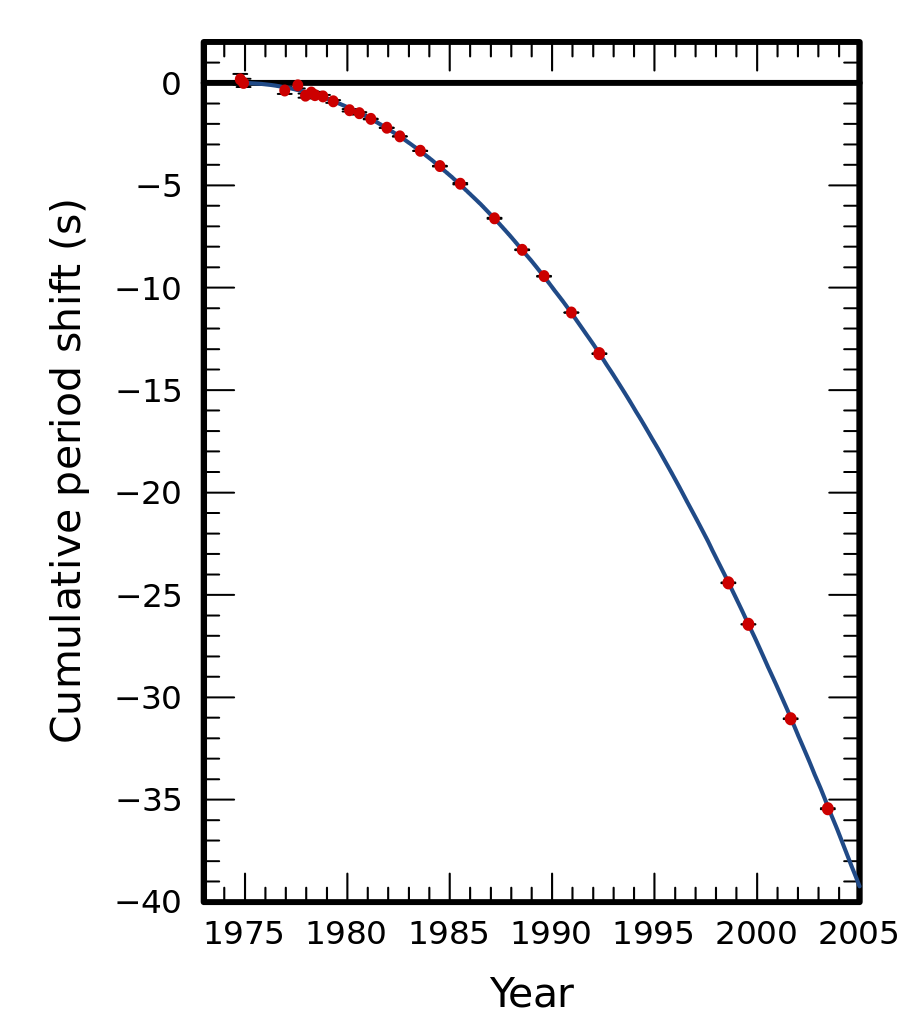
\includegraphics[width=6cm]{src/922px-PSR_B1913+16_period_shift_graph.png}
    \caption{PSR B1913+16双星的轨道周期变化. 实抛物线为广义相对论的预测而点为观测值.}
\end{figure}

对于(等质量的)双星系统, 有
\[ L = \frac{8}{5} M^2 l_0^4 \omega^6 \approx 4.0 \pare{M\omega}^{10/3}. \]
而机械能近似为
\[ E = \half M\omega^2 r^2 + \half M\omega^2 r^2 - \frac{M^2}{2r} \approx -0.40 M^{5/3}\omega^{2/3}. \]
以$T$表示双星系统的周期, 则\cite{PhysRev.136.B1224}
\[ \rec{E}\+dtdE = \frac{2}{3}\rec{\omega}\+dtd\omega = -\frac{2}{3}\rec{T}\+dtdT. \]
如果要将离心率纳入考虑, 则
\[ \expc{\+dtdE} = -\frac{32}{5}\frac{\mu\pare{m+M}^3}{a^5 \pare{1-e^2}^{7/2}}\pare{1+\frac{73}{24}e^2 + \frac{37}{96}e^4}, \]
而
\[ \expc{\+dtdT} = -\frac{192\pi}{5}\frac{\mu\pare{m+M}^{3/2}}{a^{5/2}\pare{1-e^2}^{7/2}}\pare{1+\frac{73}{24}e^2 + \frac{37}{96}e^4}. \]
对于PSR B1913+16双星(Hulse–Taylor双星)系统, 这一理论值为
\[ \+dtdT = -2.4\times 10^{-12} = \SI{-72}{\micro\second\per\year}. \]
而2004年的观测值为
\[ \+dtdT = -\pare{2.4184\pm 0.0009}\times 10^{-12}. \]
可以发现理论值和观测值吻合极好\cite{weisberg2004relativistic}.

% subsubsection 双星系统的耗散速率 (end)

% subsection 引力波的能流 (end)

% section 引力波的产生 (end)

\section{引力波的探测} % (fold)
\label{sec:引力波的探测}

\subsection{产生引力波的天体} % (fold)
\label{sub:产生引力波的天体}

\subsubsection{双星系统} % (fold)
\label{ssub:双星系统}

\begin{figure}[ht]
    \centering
    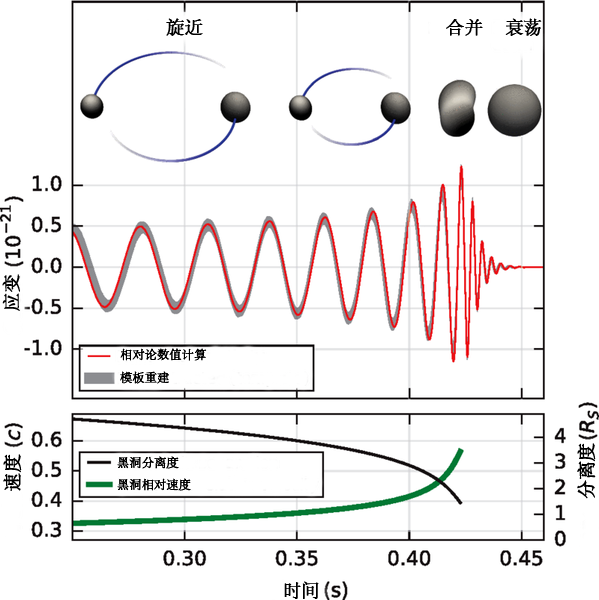
\includegraphics[width=8cm]{src/Estimated_gravitational-wave_strain_amplitude_from_GW150914(zh-hans).png}
    \caption{双黑洞合并产生的引力波信号, 可见信号频率逐渐上升}
    \label{fig:双黑洞合并产生的引力波信号}
\end{figure}

由于引力辐射损失能量, 一般的双星系统寿命近似为
\[ \tau\+_gw_ = -\frac{E}{L} = 2.43\pare{\frac{M}{M_\sun}}^{-5/3}\pare{\frac{f}{\SI{100}{\hertz}}}^{-8/3}\SI{}{\second}, \]
从而对于下限探测频率$\SI{10}{\hertz}$的探测器, 能观测到引力波的效应的时间只有数秒. 从而探测装置通常只针对双星或双黑洞合并的事件, 此时引力波的频率急剧上升, 产生啁啾信号, 可达到$\SI{2}{\kilo\hertz}$量级(如\cref{fig:双黑洞合并产生的引力波信号}). GW150914正是由双黑洞旋近, 并合以及并合后的黑洞发生的衰荡导致的.

% subsubsection 双星系统 (end)

\subsubsection{自转中子星} % (fold)
\label{ssub:自转中子星}

许多高速自转的中子星都是脉冲星. 这些中子星能够发射引力波需要以其关于旋转轴非对称为前提. 关于旋转轴对称的天体可构成Kerr黑洞, 不发生辐射. 如果中子星的质量分布并非球对称, 则可能满足这一条件. 在轻微偏离对称的情形下, 引力波的振幅大约为
\[ h \sim 2\epsilon \Omega^2 \frac{I\+_NS_}{r}. \]
其中$I\+_NS_$是中子星的转动惯量, $\epsilon$是相对自转轴的不对称率. 通过观察中子星的自转速度减小速率, 可估计引力波的能量辐射速率, 可得$\epsilon$在$10^{-3}$到$10^{-7}$量级. 从而可估计对于典型的中子星, 振幅在$10^{-25}$量级, 观测难度较大.
\par
为了观测到相应频率的引力波效应, 需要对信号做Fourier分析, 并且还需要考虑到地球自转和公转导致的Doppler效应.

% subsubsection 自转中子星 (end)

\subsubsection{引力塌缩} % (fold)
\label{ssub:引力塌缩}

超新星内核的塌缩速率极大, 且可能具有非对称性, 这一非对称性可能产生引力波. 然而由于其对内核的初始状态的敏感性, 过程的不稳定性以及对高密度物质做计算的困难性, 这类引力波的波形和振幅都难以预知. 

% subsubsection 引力塌缩 (end)

\subsubsection{宇宙大爆炸} % (fold)
\label{ssub:宇宙大爆炸}

早期的宇宙可能存在强度相当大的引力波. 随着宇宙膨胀, 这些引力波的强度逐渐衰减. 尽管其强度可能小于探测器的背景噪声的强度, 仍然可以通过比对一对探测器(例如LIGO和VIRGO)接收到的信号以确定是否存在此类引力波. 背景噪声具有相当大的随机性, 然而如果引力波的波长远大于探测器的间距, 两个探测器接受到的信号平均而言就会有非零的相关性.

% subsubsection 宇宙大爆炸 (end)

% subsection 产生引力波的天体 (end)

\subsection{探测方法} % (fold)
\label{sub:探测方法}

\subsubsection{概要} % (fold)
\label{ssub:概要}

许多天文现象都会产生引力波, 而且宇宙中只有大约$4\%$的物质由能发生电磁相互作用的带电粒子构成, 剩下的$96\%$的物质皆只能与引力场相互作用, 探测引力波将会对了解宇宙的构成和早期宇宙有重要作用. 探测机制大概有如下几种:
\begin{cenum}
    \item 共振质量探测器: 由在引力波的作用下会发生振动的振动系统构成. 这种探测器已经逐渐被精度更高的其它探测器取代.
    \item 激光干涉仪: 这种探测器使用激光探测四维固有距离的变化. LIGO, VIRGO, GEO600和TAMA300探测器皆属于此种类型.
    \item 航天器追踪: 通过地面和航天器之间通信延时的微小变化发现引力波的存在. 受制于原子钟的稳定性和太阳风的干扰, 这一机制的灵敏度不高.
    \item 脉冲星计时: 高速自转的脉冲星会以相当稳定的间隔发射电磁脉冲信号, 引力波将会对信号间隔产生围绕. 通过在地面上布置大规模的巨型射电望远镜阵(平方千米阵, Square Kilometre Array), 可以精确地测定信号间隔的变化以探测引力波.
    \item 宇宙微波背景辐射温度微扰: 大爆炸产生的引力波可能引发宇宙微波背景辐射温度的空间分布的变化, 通过测量这一变化可以探测大爆炸产生的引力波的存在.
\end{cenum}

% subsubsection 概要 (end)

\subsubsection{共振探测器} % (fold)
\label{ssub:共振探测器}

如果两个质量为$m$质点通过弹簧系数$k$, 阻尼系数$\nu$的弹簧相连接, 则自由振动时的运动方程为
\[ \xi_{,00} + 2\gamma \xi_{,0} + \omega_0^2 \xi = 0, \]
其中
\[ \xi = x_2 - x_1 - l_0,\quad \omega_0^2 = \frac{2k}{m},\quad \gamma = \frac{\nu}{m}. \]
如果有引力波通过, 则弹簧的四维固有长度会发生变化,
\[ l\pare{t} = \brac{x_2\pare{t} - x_1\pare{t}}\brac{1+\half h^{\mathrm{TT}}_{xx}\pare{t}} + O\pare{\abs{h_{\mu\nu}}^2}. \]
从而相应的伸长量应变为
\[ \xi = x_2 - x_1 - l_0 + \half \pare{x_2 - x_1} h_{xx}^{\mathrm{TT}} + O\pare{\abs{h_{\mu\nu}}^2}. \]
故运动方程变为
\[ \boxed{\xi_{,00} + 2\gamma \xi_{,0} + \omega_0^2 \xi = \half l_0 h^{\mathrm{TT}}_{xx,00}.} \]
注意到这一方程具有\textbf{受迫阻尼振动}的形式. 取
\[ h_{xx}^{\mathrm{TT}} = A\cos \Omega t, \]
有
\[ \xi = R\cos\pare{\Omega t + \phi}. \]
其中
\[ R = \frac{l_0 \Omega^2 A}{2\sqrt{\pare{\omega_0^2 - \Omega^2}^2} + 4\Omega^2\gamma^2},\quad \tan\phi = \frac{2\gamma \Omega}{\omega_0^2 - \Omega^2}. \]
简谐振子的能量为
\[ E = \half m\pare{x_{1,0}}^2 + \half m\pare{x_{2,0}}^2 + \half k\xi^2 = \rec{4}mR^2 \brac{\Omega^2 \sin^2\pare{\Omega t + \phi} + \omega_0^2 \cos^2\pare{\Omega t + \phi}}. \]
在一个周期内的平均为
\[ \expc{E} = \rec{8}mR^2 \pare{\omega_0^2 + \Omega^2}. \]
如欲设计针对某一特定频率的引力波的探测器, 则应有$\omega_0 = \Omega$, 相应的
\[ R = \rec{4}l_0 A \frac{\Omega}{\gamma},\quad E = \rec{64}ml_0^2 \Omega^2 A^2\pare{\frac{\Omega}{\gamma}}^2 = \rec{16}ml_0^2\Omega^2 A^2Q^2. \]
例如对于
\[ m = \SI{1.4e3}{\kilogram},\quad l_0 = \SI{1.5}{\meter},\quad \omega_0 = \SI{e4}{\per\second},\quad Q \approx \num{e5}, \]
以及入射引力波振幅$A \approx \num{e-20}$, 有
\[ R\approx \SI{e-15}{\meter},\quad E \approx \SI{e-20}{\joule}. \]

% subsubsection 共振探测器 (end)

\subsubsection{激光探测器} % (fold)
\label{ssub:激光探测器}

在TT规范确定的坐标系中, 对于十字形偏振的引力波, 度规为
\[ \rd{s^2} = -\rd{t^2} + \brac{1+h_+\pare{z-t}}\,\rd{x^2} + \brac{1-h_+\pare{z-t}}\,\rd{y^2} + \rd{z^2}. \]
如果两个物体分别位于$x=0$和$x=L$处, 从一个物体发射光信号经过对方物体反射后被接收, 其到达对方物体的时刻为
\[ t_1 = t_0 + \int_0^L \sqrt{1+h_+\pare{t\pare{x}}}\,\rd{x} = t_0 + L + \half \int_0^L h_+\pare{t_0 + x}\,\rd{x}. \]
从而信号被接收的时刻为
\[ t_2 = t_0 + 2L + \half \int_0^L h_+\pare{t_0 + x}\,\rd{x} + \int_0^L h_+\pare{t_0 + L + x}\,\rd{x}. \]
如果引力波的波长远大于$L$, 则在光信号传播的途中$h_+$可近似为常数, 从而总的历时正比于$L$. 对上式微分可以发现
\[ \+d{t_0}d{t_2} \approx 1 + \half \brac{h_+\pare{t_0 + 2L} - h_+\pare{t_0}}. \]
如果$t_0$时发射的是一串正弦波, 则接收的正弦波频率相对于发射频率会发生偏移,
\[ \+d{t_0}d{t_2} = \frac{\nu_2}{\nu_0}. \]
通过测量这一频移即可推知引力波的振幅. 如果引力波在$x$-$z$平面中与$z$轴成角度$\theta$传播, 则上式应替换为
\begin{equation}
    \label{eq:ThreeItems}
    \+d{t_0}d{t_2} = 1 + \half \curb{\pare{1-\sin\theta}h_+\pare{t_0 + 2L} - \pare{1+\sin\theta}h_+\pare{t_0} + 2\sin\theta h_+\pare{t_0 + \pare{1-\sin\theta} L}}.
\end{equation}

% subsubsection 激光探测器 (end)

% subsection 探测方法 (end)

\subsection{实际探测器} % (fold)
\label{sub:实际探测器}

\subsubsection{共振探测器} % (fold)
\label{ssub:共振探测器}

\begin{figure}[ht]
    \centering
    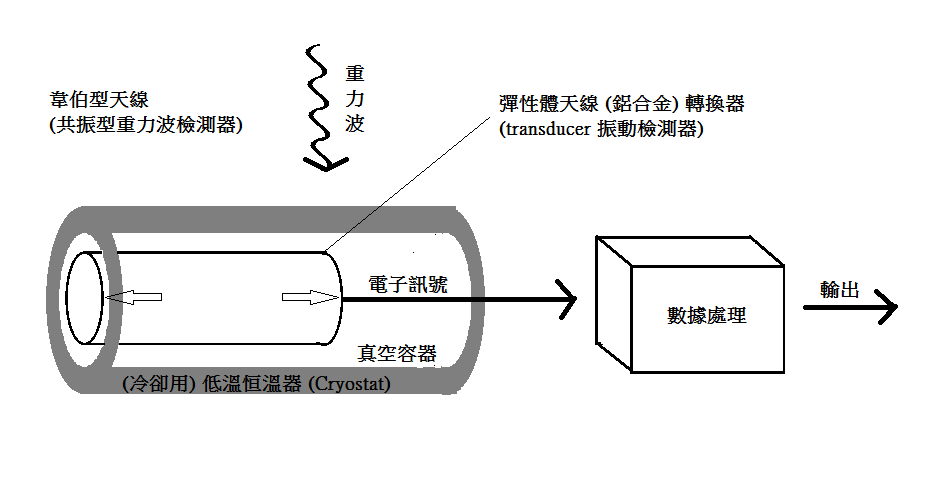
\includegraphics[width=10cm]{src/Weber_Bar.png}
    \caption{条状共振探测器}
    \label{fig:条状共振探测器}
\end{figure}

共振探测器分为条形探测器和球状探测器. 为了尽可能减小外部噪声, 例如量级在$kT$的热噪声, 需要将探测器置于极低的温度下. 目前Auriga条状探测器工作在$\SI{0.1}{\kelvin}$以下.
\par
为了防止其他噪声(例如机械振动)的干扰, 探测器会置于悬空状态, 形成一个频率极低的摆. 任何来自地面的振动可能令摆的顶端发生位移, 但只有低频的部分有可能传导到探测器, 从而有效过滤机械振动噪声.
\par
为了测量探测器的微小伸长, 早期的策略为在探测器中部放置应力传感器. 也可以将振动能量传递给极轻的, 具有共振相同频率的振动检测器(如\cref{fig:条状共振探测器}), 以获得更大的振幅.
\par
探测器的尺寸通常很小, 以免制作工艺本身导致的缺陷产生噪声. 然而振幅$10^{-21}$量级的引力波的能量可能低于一个声子, 因此探测其振动及其困难.

% subsubsection 共振探测器 (end)

\subsubsection{激光探测器} % (fold)
\label{ssub:激光探测器}

\begin{figure}[ht]
    \centering
    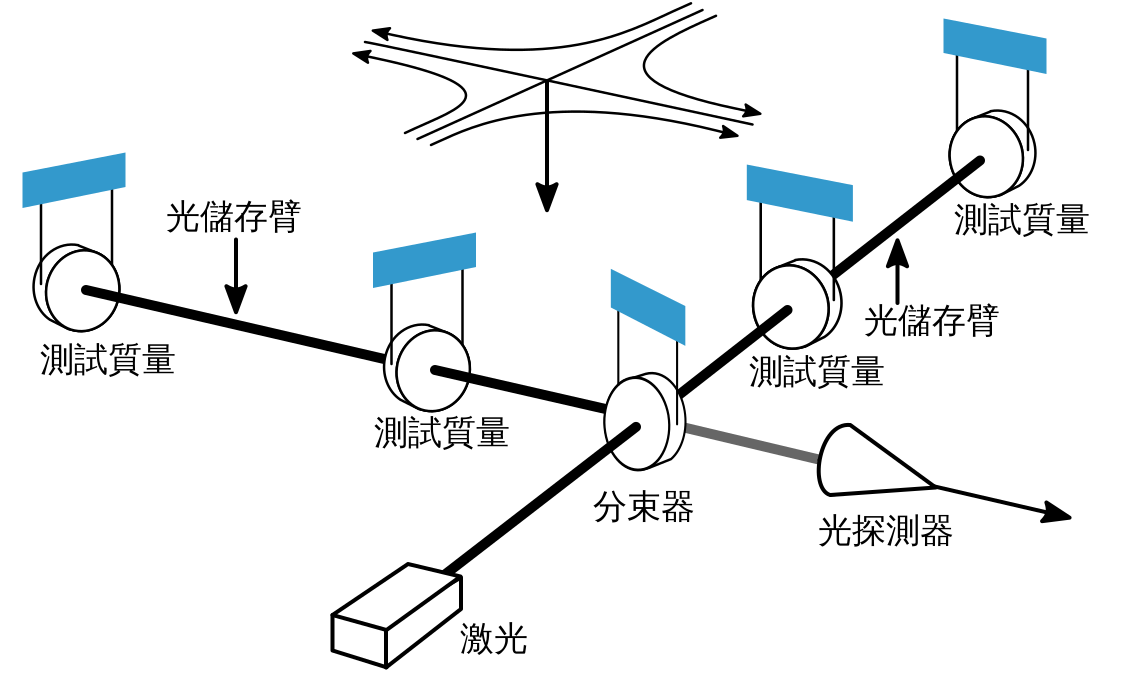
\includegraphics[width=10cm]{src/langzh-1125px-LIGO_schematic_(multilang).png}
    \caption{激光干涉探测器}
    \label{fig:激光干涉探测器}
\end{figure}

\begin{figure}[ht]
    \centering
    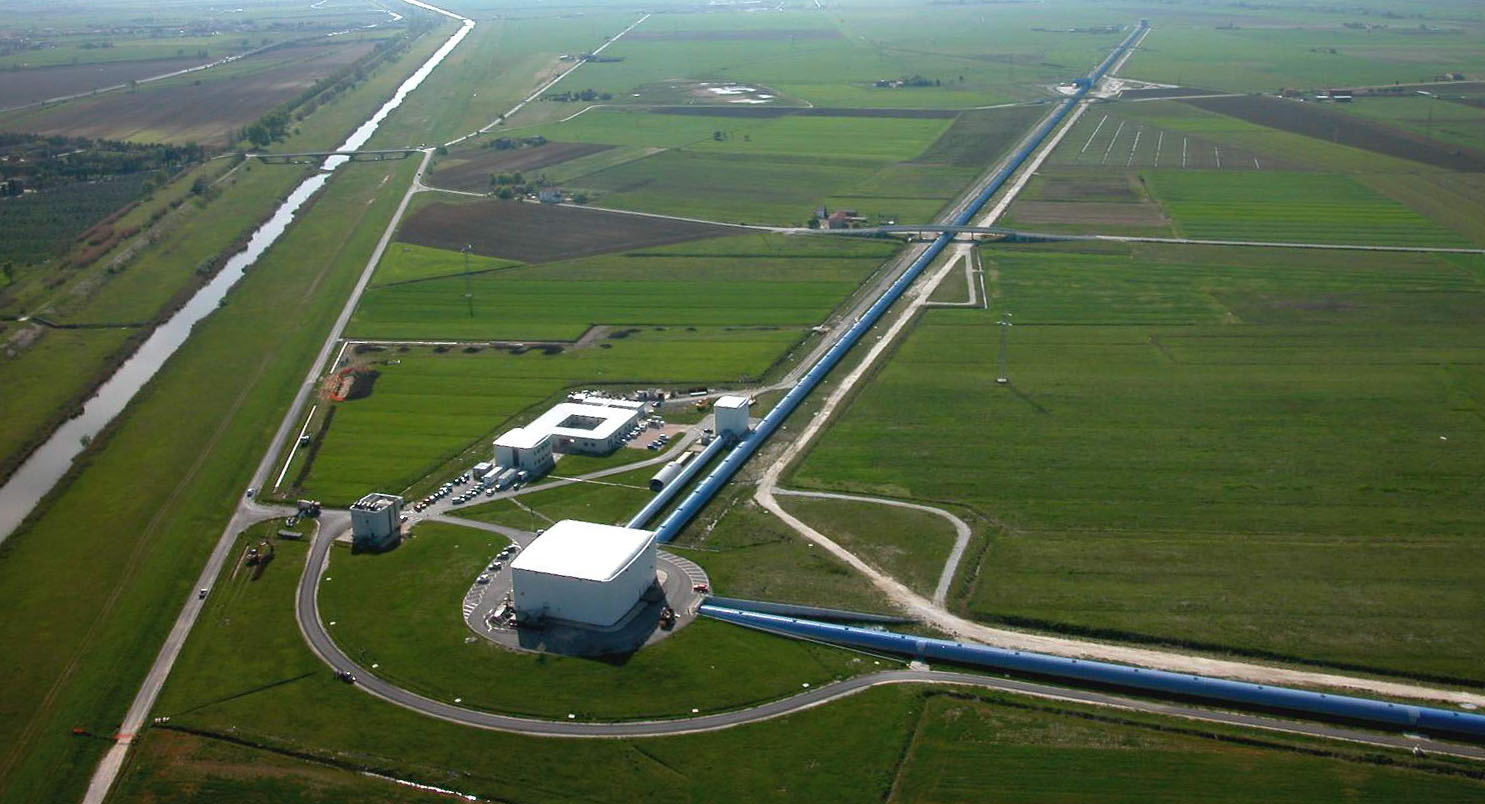
\includegraphics[width=10cm]{src/ligoandvirgo.jpg}
    \caption{VIRGO观测站, 臂长$\SI{3}{\kilo\meter}$}
    \label{fig:VIRGO观测站}
\end{figure}

最简单的激光探测器为航天器追踪探测器, 通过测量电磁波信号经过航天器反射后被接收的总历时确定其距离, 如果测量足够精确即可发现引力波产生的扰动. 为了分离星际间和电离层的折射率涨落, 需要在多处放置观测点, 并确定信号的变化满足\eqref{eq:ThreeItems}. 等离子体造成的干扰也可以通过测量多种频率的电磁波的变化分离. 然而原子钟的精度限制导致这一方法难以测量$10^{-20}$以下振幅的引力波.
\par
另一种探测器是以Michelson干涉仪为基础的探测器(如\cref{fig:激光干涉探测器}). 激光器发出的光束在两臂多次反射后入射光探测器, 两条光束会发生干涉. 如果两束光的光程完全一致, 则发生相长干涉, 探测器有信号. 如果光程相差一半波长, 则发生相消干涉, 探测器无信号. LIGO和VIRGO中两臂的长度为$\SI{3}{\kilo\meter}$至$\SI{4}{\kilo\meter}$(如\cref{fig:VIRGO观测站}), 以获得尽量显著的干涉效果.
\par
实验中的分束器, 测试质量和反射镜等皆悬空, 以减弱外部机械振动噪声产生的干扰. 热噪声则难以避免, 因为激光本身会产生相当热量, 因此现有的激光探测器大都工作在室温. 还有一种噪声源于两束激光的干涉强度的随机涨落, 这是因为发射的激光由离散的光子构成. 这种噪声是制约$\SI{200}{\hertz}$频率附近的引力波探测的主要因素. 为了减弱这种噪声, 可以在两臂的光学空腔中尽可能多地储存光子, 以减小能量涨落.
\par
虽然干涉仪已经是精密度极高的仪器, 为了提取出引力波产生的效应仍然需要恰当的数据分析. 噪声的强度通常大于引力波本身的强度, 因此为了防止噪声被误认为引力波, 需要联合不止一个探测器的数据, 在保证其皆有探测到引力波信号的前提下才能确认引力波的发生. 通过不同探测器观测到信号的时间差可以推断引力波传播的方向.
\par
除了地面上的探测器, 还有可以通过航天器上的探测器观测引力波. ESA和NASA计划通过LISA(激光干涉空间天线)在太空中观测引力波, 这可以有效过滤地球的引力场导致的噪声, 可能观测到$\SI{1}{\hertz}$以下的引力波. LISA由三个互相成等边三角形的航天器构成, 可以测量不同偏振态的引力波. 航天器间相距$\SI{5e6}{\kilo\meter}$, 较大的臂长可以有效消除热噪声的影响.
\par
LISA环绕太阳以半径$1$天文单位的轨道运行, 且与地球轨道相差$\SI{20}{\degree}$, 主要干扰来自于太阳的光压以及太阳风. 通过在航天器中放置两个不受力(从而沿测地线运动)的自由质点, 并且根据质点在航天器中位置通过动力装置微调航天器的轨道以保证航天器处于测地线轨道. 将自由质点做为激光的参考点, 可以在相当高的精度下观测引力波.

% subsubsection 激光探测器 (end)

% subsection 实际探测器 (end)

\subsection{观测到的引力波事件} % (fold)
\label{sub:观测到的引力波事件}

\subsubsection{GW150914} % (fold)
\label{ssub:gw150914}

\begin{figure}[ht]
    \centering
    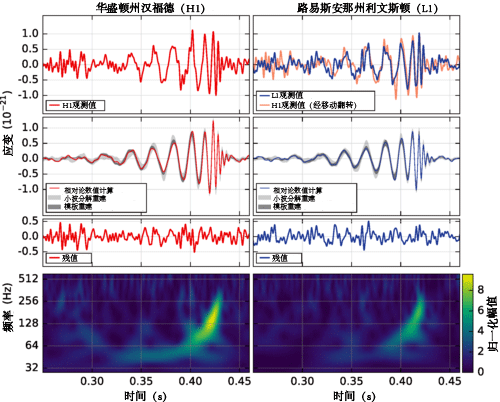
\includegraphics[width=8cm]{src/LIGO_measurement_of_gravitational_waves(zh-hans).png}
    \caption{GW150914的引力波信号\cite{PhysRevLett.116.061102}}
    \label{fig:GW150914的引力波信号}
\end{figure}

GW150914是人类历史上首次探测到的引力波. 这一事件由LIGO位于汉福德区及利文斯顿的两架探测器观测到(如\cref{fig:GW150914的引力波信号}), 信号持续时间超过$\SI{0.2}{\second}$, 并且在八个周期内频率由$\SI{35}{\hertz}$上升至$\SI{250}{\hertz}$. 通过对数据的分析可以推断引力波由两个质量分别为$36_{-4}^{+5}$和$29\pm 4$倍太阳质量的黑洞合并放出, 合并后黑洞的质量为$62\pm 4$倍太阳质量, 损失的$3.0 \pm 0.5$倍太阳质量的能量以引力波形式释放, 峰值功率$\SI{3.6e49}{\watt}$.

% subsubsection gw150914 (end)

% subsection 观测到的引力波事件 (end)

% section 引力波的探测 (end)

\bibliographystyle{unsrt}
\bibliography{Content}

\end{document}
